%%%%%%%%%%%%%%%%%%%%%%%%%%%%%%%%%%%%%%%%%%%%%%%%%%%%%%%%%%%%%%%%%%%%%%%%%%%%%%%%
%2345678901234567890123456789012345678901234567890123456789012345678901234567890
%        1         2         3         4         5         6         7         8

\documentclass[letterpaper, 10 pt, conference]{ieeeconf}  % Comment this line out if you need a4paper

%\documentclass[a4paper, 10pt, conference]{ieeeconf}      % Use this line for a4 paper

\IEEEoverridecommandlockouts                              % This command is only needed if
                                                          % you want to use the \thanks command

\overrideIEEEmargins                                      % Needed to meet printer requirements.

% See the \addtolength command later in the file to balance the column lengths
% on the last page of the document
\usepackage{amsfonts}
% The following packages can be found on http:\\www.ctan.org
\usepackage{graphics} % for pdf, bitmapped graphics files
\usepackage{multirow} % for tables
\usepackage{cite} % for bibliography
\usepackage{braket}
\usepackage{amsfonts}
\usepackage{amsmath}
\usepackage[utf8]{inputenc}
%\usepackage{subfig}
%\usepackage{amsthm}
%\usepackage{mathrsfs}
\usepackage{epsfig} % for postscript graphics files
\usepackage{nomencl}
%\usepackage{mathptmx} % assumes new font selection scheme installed
\usepackage{times} % assumes new font selection scheme installed
%\usepackage{amsmath} % assumes amsmath package installed
%\usepackage{amssymb}  % assumes amsmath package installed
\graphicspath{ {figures/} }

\title{\LARGE \bf
Scenario Risk Quantification for Automated Driving Applications
}


\author{Arash Khabbaz Saberi, Erwin de Gelder, Hala Elrofai}
%\thanks{*This research has received funding from the European Unions Horizon 2020 research and innovation programme under ROADART Grant Agreement No 636565.}% <-this % stops a space
%\thanks{$^{1}$E. van Nunen is with the Department of Integrated Vehicle Safety, TNO, P.O.
%Box 756, 5700 AT Helmond, The Netherlands, and also with the Department of Mechanical Engineering, Eindhoven University of Technology, 5600 MB Eindhoven, The Netherlands
%{\tt\small ellen.vannunen@tno.nl}}


\begin{document}



\maketitle
\thispagestyle{empty}
\pagestyle{empty}


%%%%%%%%%%%%%%%%%%%%%%%%%%%%%%%%%%%%%%%%%%%%%%%%%%%%%%%%%%%%%%%%%%%%%%%%%%%%%%%%
\begin{abstract}
This paper aims to answer the question how relevant the use case of emergency braking of a lead vehicle in a platoon is in combination with a V2V failure. This combination is very hazardous and is likely to lead to a collision, but the probability that both of these events occur at the same time is very small. Should this worst-case use case be considered in the design and function definition of a platooning application? Further, this paper aims to propose how to set up an approach to answer this question.
\end{abstract}


%%%%%%%%%%%%%%%%%%%%%%%%%%%%%%%%%%%%%%%%%%%%%%%%%%%%%%%%%%%%%%%%%%%%%%%%%%%%%%%%
\section{INTRODUCTION}
TODO

\section{DEFINITIONS} % Erwin (use the other paper) & Arash

TODO: give more examples
First, we introduce the following notions:
\begin{enumerate}
\item{Risk = Severity $\times$ Probability  }
\item{Severity: a quantitative measure, depending on the impact velocity.}
\item{Event: actor performing a action during a certain time period.}
\item{Action: the relevant actions here are braking, and failure.  }
\item{Actor: the relevant actors here are the lead vehicle (denoted with L), the following vehicle (F) and the communication unit (V2V)}
\item{Intended acceleration,  the control output which will be realized by the driveline of either the lead, denoted by $u_L$, or the follower, denoted by $u_F$.}
\end{enumerate}



\section{PROBLEM DEFINITION}\label{sec:problem} % Arash
The need for quantification on risk calculation for automated driving. 
TODO: formalizing this senctence in the context of scenario. 

Differentiating probability of a single (hazardous) event (state of art) to what we are doing: i.e. probability of whole scenario. 

\section{Proposed Risk Estimation Method} % Arash & Hala


\begin{enumerate}
	\item Back ground on risk (ISO 26262/SOTIF) and acceptable level of risk
	\item High level description of the method 
	\item explaining how assumptions are being made
\end{enumerate}


\begin{enumerate}
\item{Compare the risk of the platooning driving behavior ($R_p$)to the risk of human drivers ($R_h$) with respect to rear-end-collisions only. If $$R_p < \frac{1}{10} R_h, $$ the risk is assumed to be acceptable.}
\item{For calculating the risk of the autonomous driving behavior with respect to rear-end-collisions only, we list the relevant events as follows:
\begin{enumerate}
\item{E1: V2V Failure, for $t\in[t_{E1}, t_{E1}+\Delta t_{E1}]$}
\item{E2: Lead performs an emergency brake with $u_{L}(t)\leq u_1$ , for $t\in[t_{E2}, t_{E2}+\Delta t_{E2}]$}
\item{E3: The CACC controller of the follower vehicle reacts to the emergency brake (by braking) at $t\in[t_{E3}, t_{E3}+\Delta t_{E3}]$.}
\item{E4: Collision occurs with an impact speed higher than 10~kph.}
\end{enumerate}
}
\item{We calculate the total probability of these events to lead to a collision as:
\begin{equation}
P_{tot} = P(E1) \times P(E2|E1) \times P(E3|E2) \times P(E4|E3)
\end{equation}
Note that potentially the V2V failure will occur later than the brake action of the lead, (in which case $t_{E2}<t_{E1}$). However, since these events are independent, this does not have any consequences for the proposed approach. Also, due to its independency $ P(E2|E1)=P(E2)$.
Now, we assume that the controller will respond to it (although it may respond late, it will respond eventually), so $P(E3|E2)=1$. Further, let us assume that we can identify a convex set $\mathcal{S}$ for which all states lead to collision with an impact speed higher than 10~kph, than $P(E4|E3)=1$.  Now only the probability of states in this set needs to be calculated.
This collision set $\mathcal{S}$ includes states related to timings as well as initial conditions. We define state $x$ as
\begin{eqnarray*}
x&=&\{(t_{E1},\Delta t_{E1},u_{1},t_{E2},\Delta t_{E2},\\
&&d_i(t_{E2}),v_i(t_{E2}),a_i(t_{E2}), v_{i-1}(t_{E2}),a_{i-1}(t_{E2})) \}
\end{eqnarray*}
and $\mathcal{S} = \{x \in \mathbb{R}^9|x_L < x < x_U\}$ with $x_L \in \mathbb{R}^9$ the lower bound and $x_U \in \mathbb{R}^9$ the upper bound. }
\item{Now the risk can be calculated as $P_{tot} \times $...TODO? (ARASH)}
\end{enumerate}

\section{Case Study} % Erwin & Hala

\begin{enumerate}
	\item use case description
	\item specific assumptions for this case
	\item description of the models used for calculating the probabilities 
	\item 
\end{enumerate}


This section details the models applied to derive the probabilities
\subsection{COLLISION SET}
This section aims to identify the set $\mathcal{S}$. I'm crossing my fingers that this will be a convex set ;)
As an example we have Fig.~\ref{fig:example}, which identifies possible collisions for $u_L<-5 m/s^2$ AND ...
(ELLEN)
\begin{figure}
  \centering
  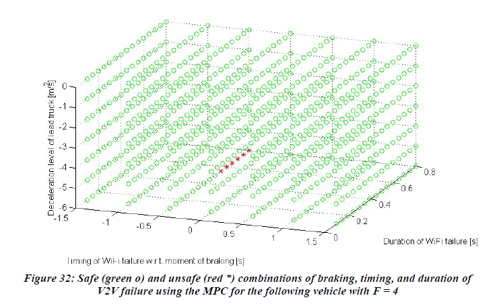
\includegraphics[width=1\columnwidth]{example.png}
  \caption{Example }\label{fig:example}
\end{figure}


\section{DISCUSSION AND FUTURE OUTLOOK} % Hala & Erwin & Arash

\section{CONCLUSIONS}\label{sec:conc}




\section*{ACKNOWLEDGEMENT}

%%%%%%%%%%%%%%%%%%%%%%%%%%%%%%%%%%%%%%%%%%%%%%%%%%%%%%%%%%%%%%%%%%%%%%%%%%%%%%%%


%\bibliography{mybib}
%\bibliographystyle{ieeetr}


\end{document}
